% !TeX spellcheck = pt_PT
% !TeX encoding = UTF-8
\documentclass[a4paper,titlepage]{article}

\usepackage[utf8]{inputenc}
\usepackage[portuguese]{babel}
\usepackage{hyperref}
\usepackage{listingsutf8}
\usepackage{float}
\usepackage{color}
\usepackage[usenames,dvipsnames]{xcolor}
\usepackage{graphicx}
% \usepackage{indentfirst}
%\usepackage{epstopdf}
\usepackage{eurosym}
\usepackage{tabularx}
\usepackage{svg}
\usepackage{fancyhdr}
\usepackage{pdfpages}

% Uma forma de usar caracteres especiais nos ficheiros de código-fonte.
\lstset{literate=%
 {á}{{\'a}}1 {é}{{\'e}}1 {í}{{\'i}}1 {ó}{{\'o}}1 {ú}{{\'u}}1
   {Á}{{\'A}}1 {É}{{\'E}}1 {Í}{{\'I}}1 {Ó}{{\'O}}1 {Ú}{{\'U}}1
   {à}{{\`a}}1 {è}{{\'e}}1 {ì}{{\`i}}1 {ò}{{\`o}}1 {ò}{{\`u}}1
   {À}{{\`A}}1 {È}{{\'E}}1 {Ì}{{\`I}}1 {Ò}{{\`O}}1 {Ò}{{\`U}}1
   {ä}{{\"a}}1 {ë}{{\"e}}1 {ï}{{\"i}}1 {ö}{{\"o}}1 {ü}{{\"u}}1
   {Ä}{{\"A}}1 {Ë}{{\"E}}1 {Ï}{{\"I}}1 {Ö}{{\"O}}1 {Ü}{{\"U}}1
   {â}{{\^a}}1 {ê}{{\^e}}1 {î}{{\^i}}1 {ô}{{\^o}}1 {û}{{\^u}}1
   {Â}{{\^A}}1 {Ê}{{\^E}}1 {Î}{{\^I}}1 {Ô}{{\^O}}1 {Û}{{\^U}}1
   {œ}{{\oe}}1 {Œ}{{\OE}}1 {æ}{{\ae}}1 {Æ}{{\AE}}1 {ß}{{\ss}}1
   {ç}{{\c c}}1 {Ç}{{\c C}}1 {ø}{{\o}}1 {å}{{\r a}}1 {Å}{{\r A}}1
   {õ}{{\~{o}}}1
   {ã}{{\~a}}1
   {€}{{\EUR}}1 {£}{{\pounds}}1
}

%\hypersetup{
%    colorlinks = false,
%    hidelinks
%}

\lstdefinelanguage{ios} {
	morekeywords={enable, interface, exit, no, ip, ipv6, network, dhcp, pool, configure, address, shutdown, route, console, terminal, nd, prefix, tunnel, source, destination, secret, line, password, login, banner, motd, hostname, end, vty, mode, gre, transport, input, router, ospf},
	otherkeywords={default-router, excluded-address, domain-lookup, unicast-routing}, % multi-word keywords! :)
	sensitive=true,
	morecomment=[l]{!}
}

\lstdefinestyle{ioscommands} {
  belowcaptionskip=1\baselineskip,
  breaklines=true,
  breakatwhitespace=true,
  xleftmargin=\parindent,
  extendedchars=true,
  language=ios,
  captionpos=b,
  numbersep=5pt,
  basicstyle=\footnotesize,
  keywordstyle=\bfseries\color{blue},
  commentstyle=\itshape\color{CadetBlue},
  identifierstyle=\color{black},
  frame=single,
  tabsize=2
}

\lstdefinestyle{bare} {
  belowcaptionskip=1\baselineskip,
  breaklines=true,
  breakatwhitespace=true,
  xleftmargin=\parindent,
  extendedchars=true,
  language=ios,
  captionpos=b,
  numbersep=5pt,
  basicstyle=\footnotesize,
  keywordstyle=\footnotesize,
  commentstyle=\footnotesize,
  identifierstyle=\footnotesize,
  frame=single
}

\title{PROJECTO DE REDES 2012 / 2013}

\pagestyle{fancy} %estilo fancy

\lhead{}
 
%\lhead{\rightmark} %escrever na esquerda do cabeçalho
 
%\chead{} %escrever no centro do cabeçalho
 
\rhead{Trabalho Prático Nº3} % escrever na direita do cabeçalho
 
\lfoot{Projecto de Redes - 2013/2014} %escrever na esquerda do rodapé
 
\cfoot{} %escrever no centro do rodapé
\rfoot{\thepage} % escrever na direita do rodapé

\author{
	Dário Jorge  nº 17104\\
	Bruno Calças nº 11598\\
}

\date{Abril de 2014}

\begin{document}

	\maketitle
	
	\newpage
	
	\tableofcontents
	
	\newpage
	
	\section{Objectivos}
		Montagem da componente física de uma rede.\\
		Configuração de equipamento activo.\\
		Autenticação 802.1x.\\
		Proxy Radius.\\
		Debugging e trobleshooting.\\
	\section{Topologia}
		\begin{figure}[H]
			\centering
			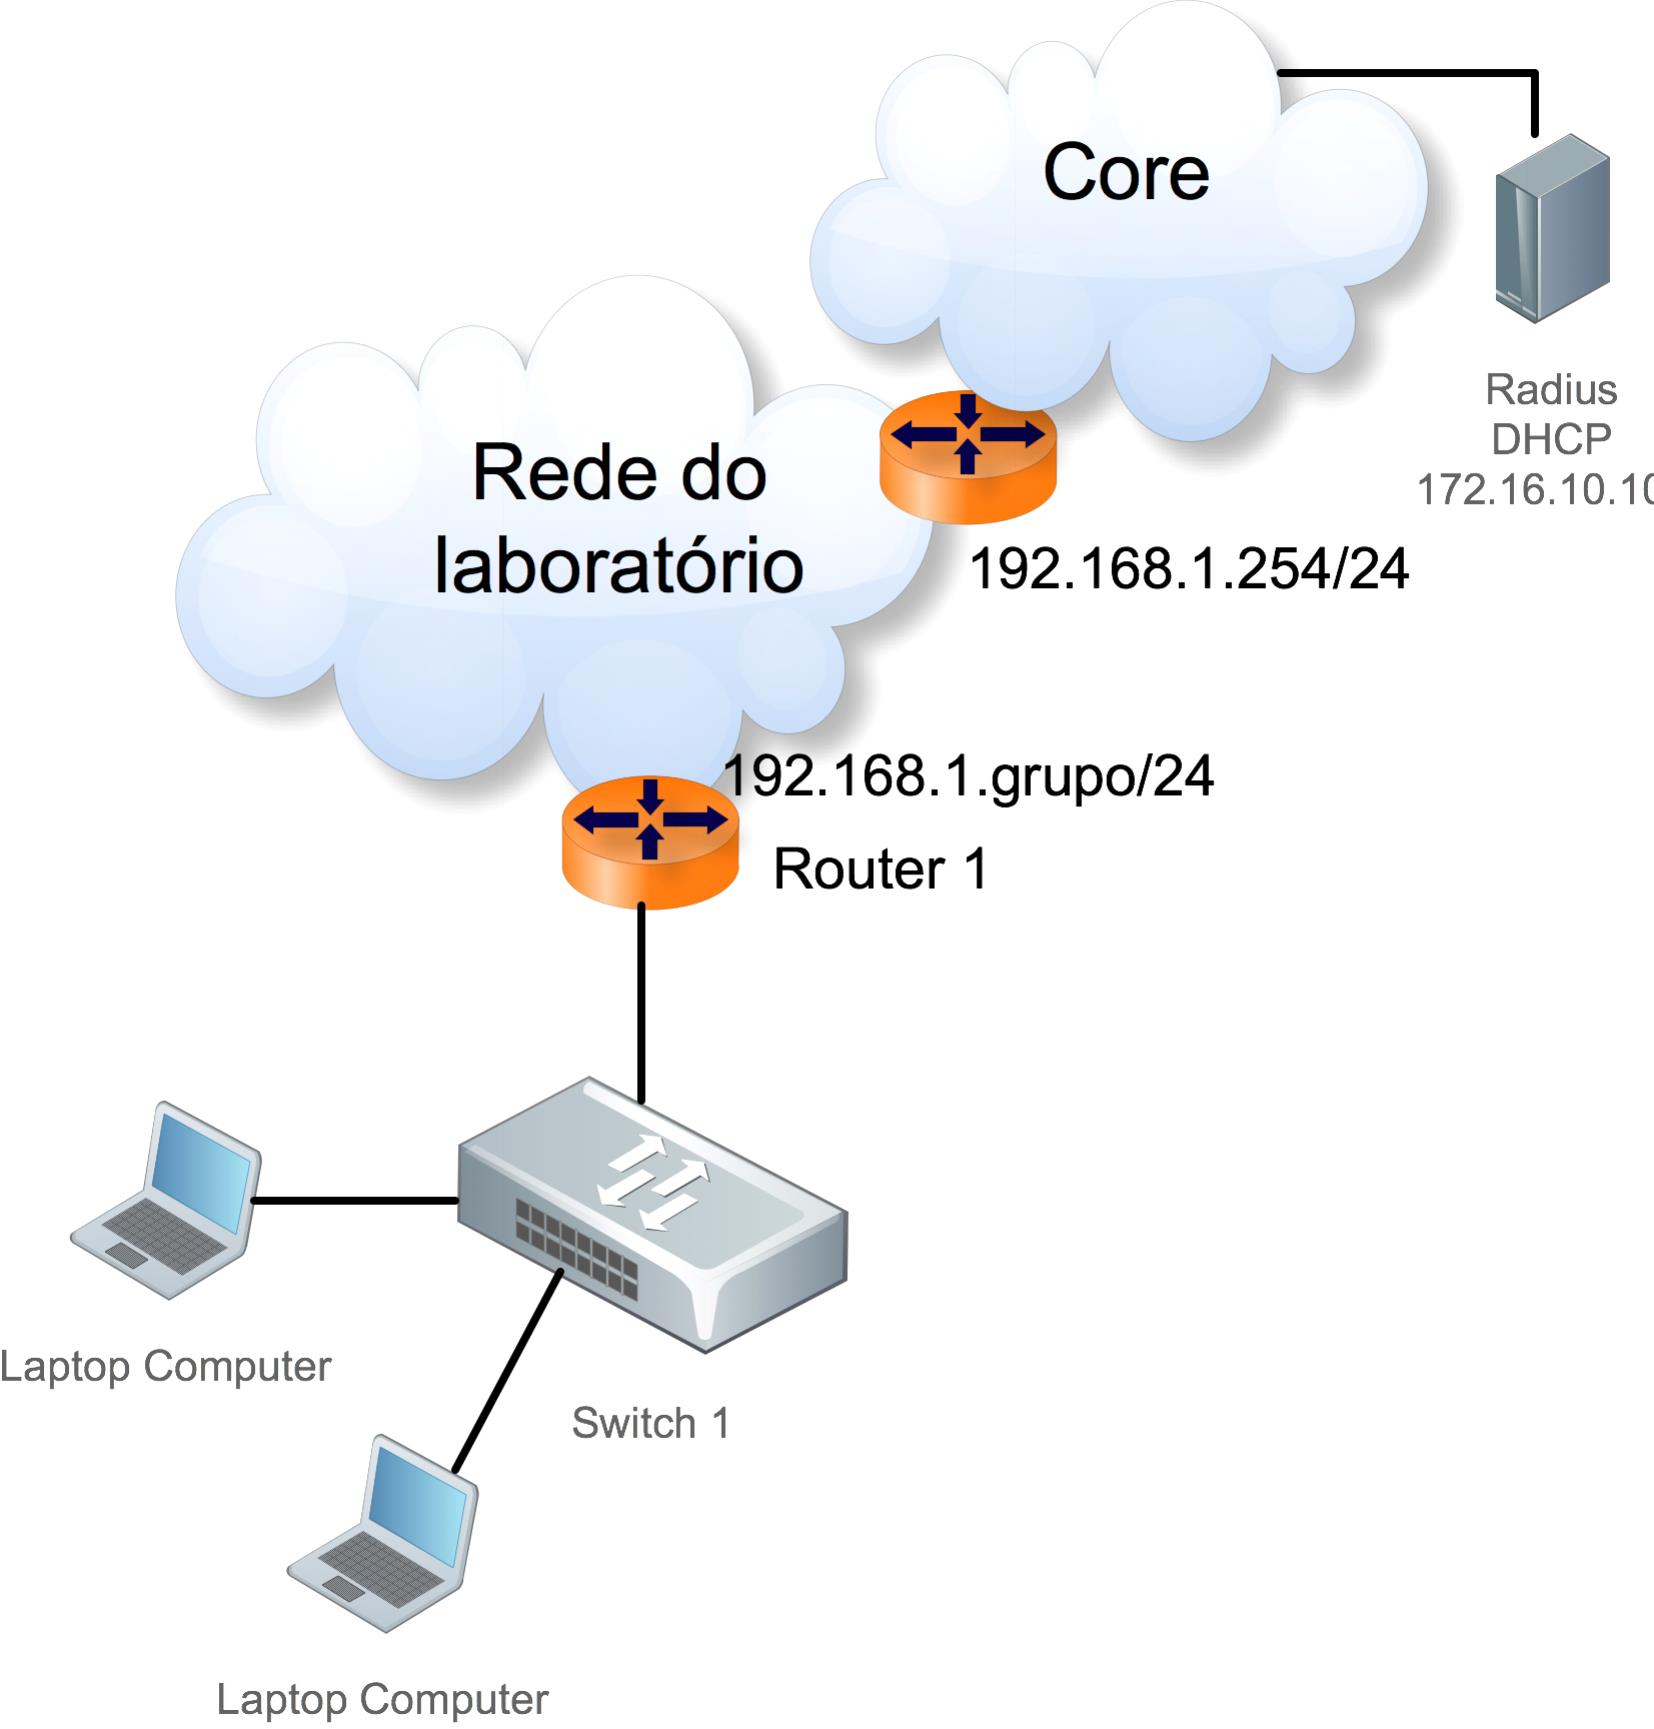
\includegraphics[width=\linewidth]{topologia.jpg}
			\caption{Topologia do trabalho}
		\end{figure}
	\section{Tabela das Vlans}
		\begin{tabular}{|c|c|c|c|c|}
			\hline Vlan ID & Nome & Portas & Modo & Default Gateway dos membros dessa Vlan\\
			\hline
			99 & Gestão & Fa 0/24 & tagged & 10.99.grupo.254\\ 
			\cline{3-4} && Mgmt & N/A &\\ \hline
			10 & Funcionários & Fa 0/24 & tagged & 10.100.grupo.254\\ 
			\cline{3-4} && Fa 0/0-12 & untagged &\\ \hline
			20 & Alunos & Fa 0/24 & tagged & 10.200.grupo.254\\ 
			\cline{3-4} && Fa 0/13-16 & untagged &\\ \hline
			30 & guest & Fa 0/17-20 & untagged & N/A\\
			\hline
			\end{tabular}
	\section{Configurações}
			\subsection{Configurações iniciais}
				- Apagar as configurações iniciais do router e do switch\\
				\lstinputlisting[style=bare]{ConfigsInit.txt}
			\subsection{Configurações básicas}
						Configure o Router de acordo com as orientações seguintes:\\
						1. Atribua um nome a cada router de acordo com a topologia descrita (hostname)\\
						2. Desabilite o DNS lookup.\\
						3. Configure uma password para aceder ao modo Exec Privileged Mode.
						(Password=class)\\
						4. Configure a message-of-the-day banner.\\
						5. Configure uma password para ligações do tipo console. (Password=class)\\
						6. Configure uma password para ligações do tipo VTY. (Password=class)\\
					
						\lstinputlisting[style=bare]{ConfigsBasic.txt}
			\subsection{Configuração do Router e do Switch.}
						\subsubsection{Configuração do Router}
							\lstinputlisting[style=bare]{ConfigsIntRouter.txt}
						\subsubsection{Configuração do Switch}
							\lstinputlisting[style=bare]{switchConfigs.txt}
			\subsection{visualisação das configurações do switch e do router}
						\subsubsection{Router}
							\lstinputlisting[style=bare]{RouterConfigsC.txt}
						\subsubsection{Switch}
							\lstinputlisting[style=bare]{SwitchCorrigido.txt}
	\section{Demonstrações}
			\subsection{Demonstração Radius}
						\begin{figure}[H]
								\centering
								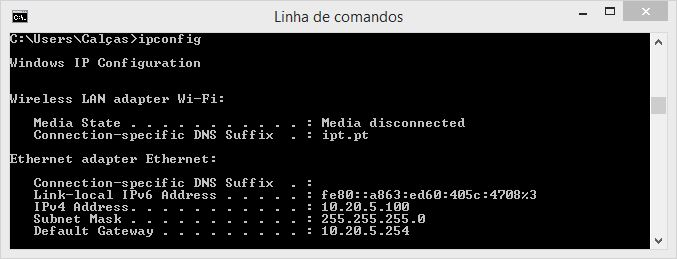
\includegraphics[width=\linewidth]{RADIUS_IP.jpg}
								\caption{Ip fornecido pelo servidor Radius}
						\end{figure}
						Demonstração do servidor radius a funcionar.\\
						\lstinputlisting[style=bare]{demonstracaoRadius.txt}
			\subsection{Ip's e Interfaces do ebits}
					\subsubsection{Interface ebits}
						\begin{figure}[H]
								\centering
								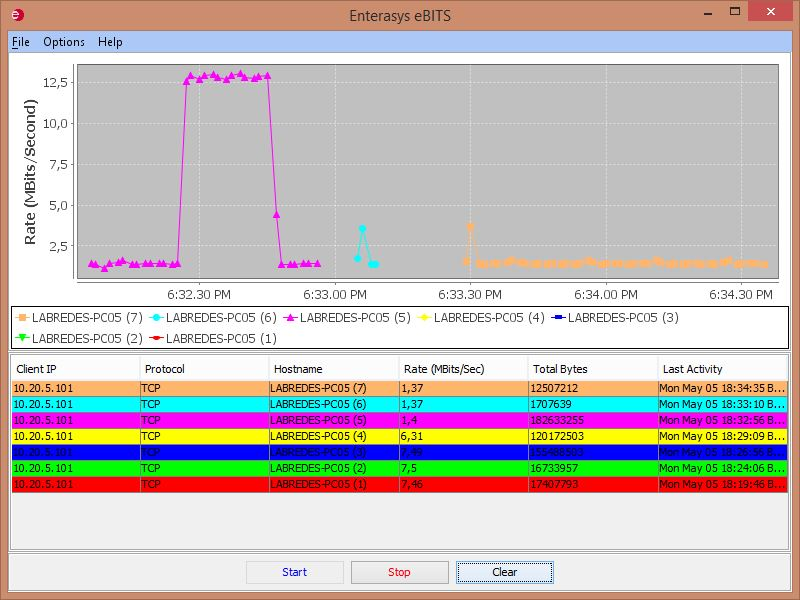
\includegraphics[width=\linewidth]{ebits_servidor.jpg}
								\caption{Servidor ebits a enviar pacotes}
						\end{figure}
						\begin{figure}[H]
								\centering
								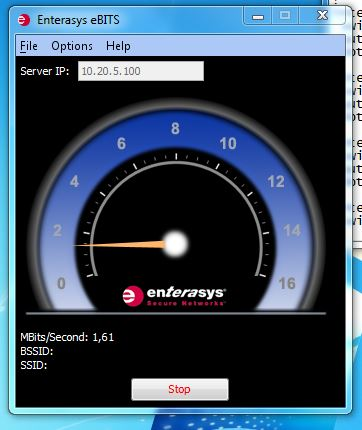
\includegraphics[width=\linewidth]{ebits-rate-limiting.jpg}
								\caption{Rate limiting a funcionar}
						\end{figure}
					\subsubsection{Ip cliente e servidor}
						\begin{figure}[H]
								\centering
								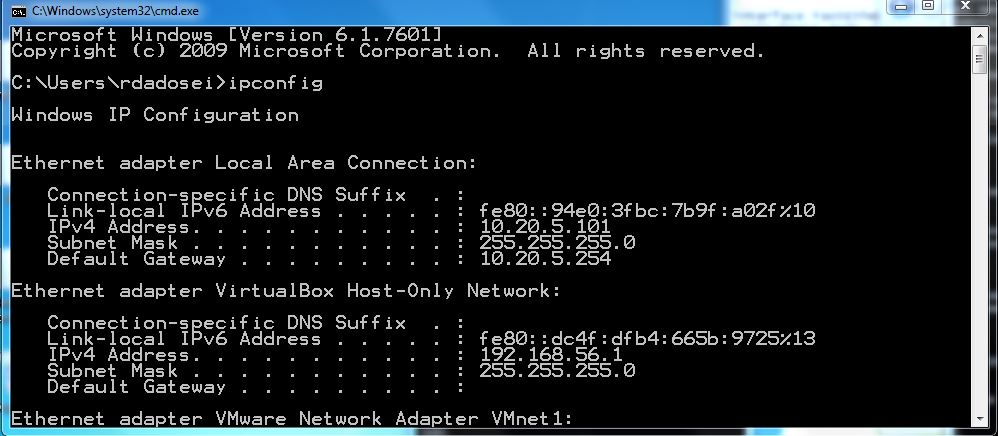
\includegraphics[width=\linewidth]{ipCliente.jpg}
								\caption{ip do cliente que irá usar o ebits}
						\end{figure}
						\begin{figure}[H]
								\centering
								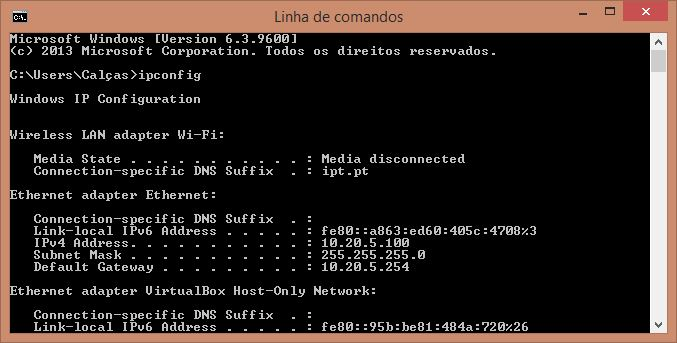
\includegraphics[width=\linewidth]{ipServidor.jpg}
								\caption{ip do servidor que irá enviar os pacotes}
						\end{figure}
			
\end{document}
